\section{Nutzerstudien}
\subsection{Think Aloud}
Die Think Aloud Nutzerstudie fand im Rahmen der Nutzerstudien statt. Hierbei wurden vier Testpersonen unabhängig voneinander Aufgaben gestellt,
welche diese auf der Webseite bewältigen sollten. Dabei sollten die Testpersonen ihre Gedanken und Tätigkeiten laut mit dem Leiter des Testes teilen.
In anbetracht gezogen wurden hierbei die technischen Kenntnisse der Testpersonen und das benutze Endgerät mit Browser. Im folgenden werden die Ergebnisse zusammengefasst.
Gestellte Aufgaben:

\textbf{Finden Sie einen beliebigen Sensor und finden Sie die aktuellen Luftfeuchtigkeitswerte dieses Sensors heraus.}

Bei dieser Aufgabe haben sich alle Testpersonen gleich verhalten. 
Aufgabe erfüllt durch klicken einen der Sensoren in Augsburg.

\textbf{Finden Sie den Sensor in Gamisch-Partenkirchen und finden Sie heraus welche Werte dieser Sensor misst.}

Bei dieser Aufgabe haben sich alle Testpersonen gleich verhalten. 
Aufgabe erfüllt durch benutzen der Suchleiste, klicken auf Suchen und anschließendes klicken auf den Sensor.

\textbf{Aktivieren Sie die Hilfe und den Experten-Modus.}

Die Hilfe wurde von den Testpersonen nach kurzen Suchen gefunden.
Bei der Aktivierung des Experten-Modus war unklar was dieser macht. Nach einigem Suchen haben die Testpersonen erkannt das dieser in der Sensoroverview weitere Daten anzeigt.
Aufgrund dessen wurden an einigen Stellen auf der Webseite weitere Hilfen verteilt, welche Unklarheiten beseitigen sollen. 

\textbf{Finden Sie den berechneten/interpolierten Wert für die Temperatur an einem beliebigen Punkt heraus.}

Unklarheiten durch das benutzen des Wortes \enquote{Interpoliert}. Testpersonen wussten nicht was gemeint war. Nach einer kurzen Aufklärung war Ihnen bewusst
was gemeint war. 
Zuerst gesucht in dem weitere Funktionen-dropdown. Das interpolierte Overlay wurde dann in Ansichten gefunden.
Aufgrund dessen wurde das interpolierte Overlay umbenannt. 

\subsection{Zusammenfassung des Think Aloud}
Durch die Auswertung der Think Aloud Benutzerstudie wurden Änderungen bezüglich der Benennung von Funktionen durchgeführt. Außerdem wurden mehr Hilfe Popups hinzugefügt damit auch Benutzer mit weniger
technischen Kenntnissen die Seite problemlos benutzen können.

\subsection{Nutzerstudie nach dem Sus-Prinzip}
Die Nutzerstude wurde mit 12 Testpersonen durchgeführt, welche an die Sus Nutzerstudie angelehnt wurde. 
Bei den Teilnehmern der Nutzerstude handelt es sich um Freunde und Bekannte mit unterschiedlichen technischen Kenntnissen. 
Hierbei wurden die allgemeine Benutzbarkeit der Webseite sowohl auch die Ladezeiten betrachtet und ausgewerte
Bei beiden Einschätzungen wurde eine Skala von 1 bis 5 verwendet, wobei 1 für \enquote{Stimme überhaupt nicht zu} und 5 für \enquote{Stimme voll zu} steht.

Im folgenden werden die Ergebnisse vorgestellt.
\subsubsection{Allgemeine Benutzung der Seite}
\begin{figure}[H]
    \centering
    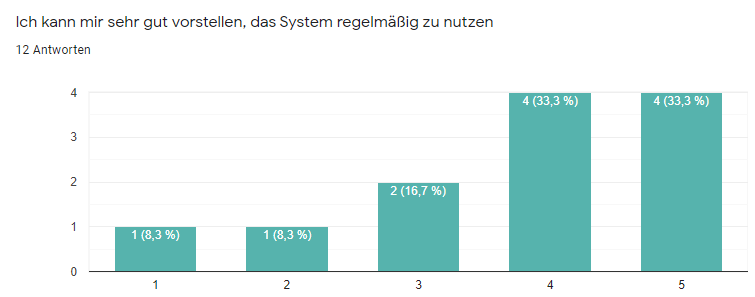
\includegraphics[width=0.7\textwidth]{media/survey/regularUsage.png}
\end{figure}
Die weniger positiven Bewertungen stammen vermutlich davon, dass weniger Interesse bezüglich Luftqualitätsdaten besteht.

\begin{figure}[H]
    \centering
    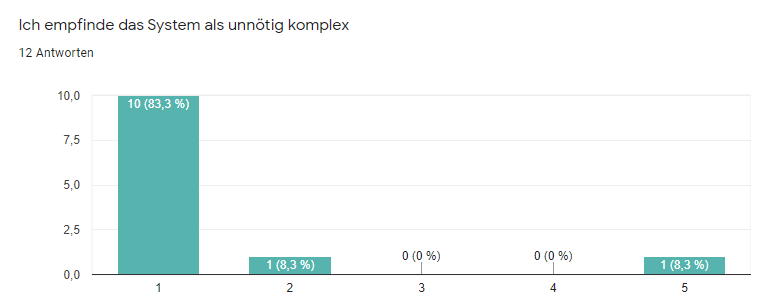
\includegraphics[width=0.7\textwidth]{media/survey/complexity.png}
\end{figure}

\noChanges

\begin{figure}[H]
    \centering
    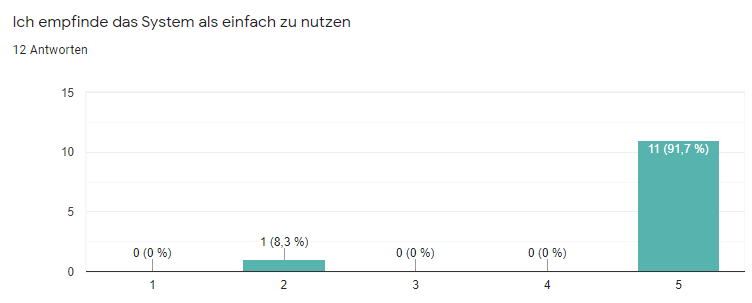
\includegraphics[width=0.7\textwidth]{media/survey/easyUsage.png}
\end{figure}

\noChanges

\begin{figure}[H]
    \centering
    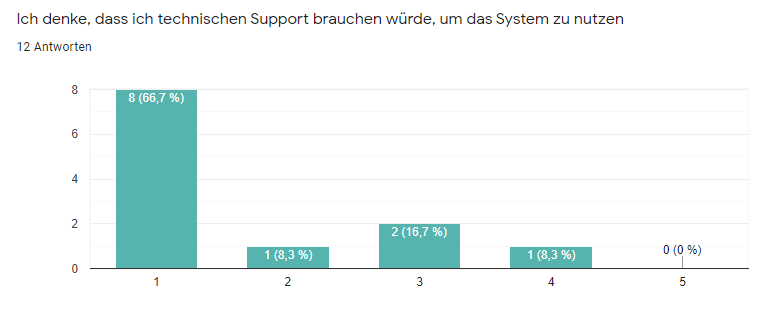
\includegraphics[width=0.7\textwidth]{media/survey/technicalSupport.png}
\end{figure}

\noChanges

\begin{figure}[H]
    \centering
    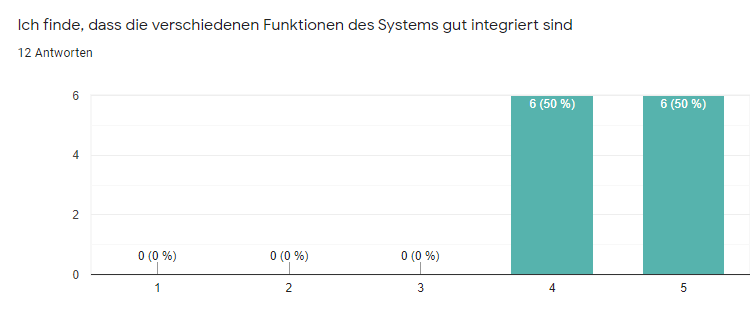
\includegraphics[width=0.7\textwidth]{media/survey/integrity.png}
\end{figure}

\noChanges

\begin{figure}[H]
    \centering
    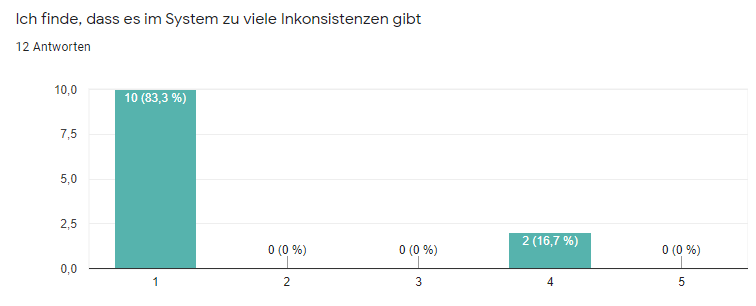
\includegraphics[width=0.7\textwidth]{media/survey/inconsistent.png}
\end{figure}

\noChanges

\begin{figure}[H]
    \centering
    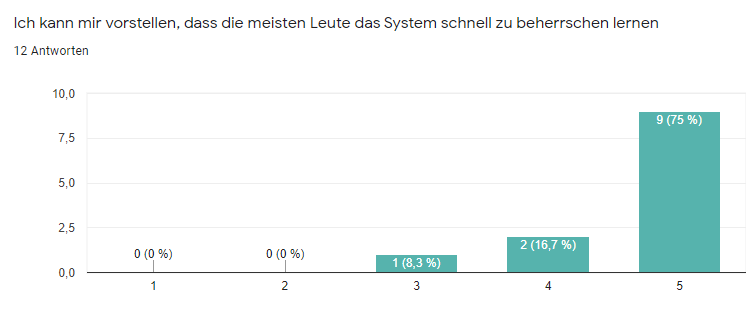
\includegraphics[width=0.7\textwidth]{media/survey/fastLearning.png}
\end{figure}

\noChanges
\begin{figure}[H]
    \centering
    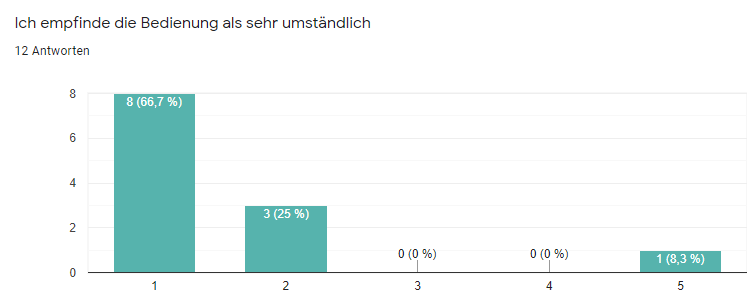
\includegraphics[width=0.7\textwidth]{media/survey/overelaboratedInterface.png}
\end{figure}

\noChanges
\begin{figure}[H]
    \centering
    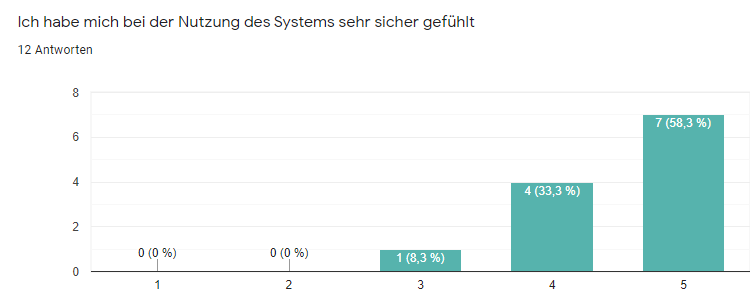
\includegraphics[width=0.7\textwidth]{media/survey/safeUsage.png}
\end{figure}

\noChanges
\begin{figure}[H]
    \centering
    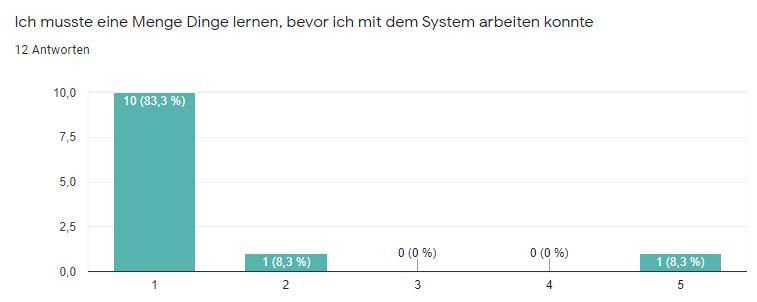
\includegraphics[width=0.7\textwidth]{media/survey/needToLearnUsage.png}
\end{figure}

\noChanges

Zusammengefasst ergibts ich ein gutes Ergebniss bezüglich der allgemeinen Benutzung der Seite und keine ausschlaggebenden Änderungen.
\subsubsection{Allgemeine Laufzeit der Seite}
Hierbei wurde nach der allgemeinen Warte- und Laufzeit gefragt. Diese wurde von den Teilnehmern als nicht störrend oder unangenehm lang wahrgenommen.
Zusammengefasst ergab sich für die drei Fragen hierbei ein sehr gutes Bild. 

\subsubsection{Freie Antwortmöglichkeiten}
Die freien Antwortmöglichkeiten ergaben, dass die Nutzer zufrieden mit der Webseite sind. 
Eine Antwort ergab, dass es eine Barriere bezüglich Farbenblindheit gab.
Dies führte dazu, dass der in den Wunschkriterien erwähnten und später verworfenen Farbenblind-Modus doch einführt wurde. 

\subsection{Zusammenfassung der Nutzerstudie nach Sus}

Die Nutzerstudie ergab das wenig Änderungen an der Webseite durchgeführt werden mussten.
